
%(BEGIN_QUESTION)
% Copyright 2006, Tony R. Kuphaldt, released under the Creative Commons Attribution License (v 1.0)
% This means you may do almost anything with this work of mine, so long as you give me proper credit

{\it Strain gauges} may be used to measure the weight of a process vessel, and therefore infer the level of fluid or solids in that vessel.  Strain gauge circuits almost always take the form of a Wheatstone bridge, the bridge circuit producing an output voltage that varies with the amount of strain sensed by the gauge:

$$\includegraphics[width=15.5cm]{i00038x01.eps}$$

Assume that the bridge is balanced when the vessel is empty (zero level), and that the resistance of the strain gauge increases with increasing vessel weight (increasing level).  Identify:

\begin{itemize}
\item{} The polarity of the voltage across all bridge resistors.
\item{} The polarity of the voltage sensed by the measuring instrument as level increases.
\item{} Which variable resistance ($R_1$ or $R_2$) adjusts {\it zero}.
\item{} Which variable resistance ($R_1$ or $R_2$) adjusts {\it span}.
\item{} One electrical fault resulting in a positive over-range ($>$ 100 \% level) reading.
\item{} One electrical fault resulting in a negative over-range ($<$ 0 \% level) reading.
\end{itemize}

\vfil 

\underbar{file i00038}
\eject
%(END_QUESTION)





%(BEGIN_ANSWER)

This is a graded question -- no answers or hints given!

%(END_ANSWER)





%(BEGIN_NOTES)

\begin{itemize}
\item{} The polarity of the voltage across all bridge resistors: {\it tops positive, bottoms negative} 
\item{} The polarity of the voltage sensed by the measuring instrument as level increases: {left positive and right negative}
\item{} Which variable resistance ($R_1$ or $R_2$) adjusts {\it zero}: {\it $R_2$}
\item{} Which variable resistance ($R_1$ or $R_2$) adjusts {\it span}: {\it $R_1$}
\item{} One electrical fault resulting in a positive over-range ($>$ 100 \% level) reading: {\it $R_{strain}$ or $R_2$ open ; $R_1$ or $R_3$ shorted}
\item{} One electrical fault resulting in a negative over-range ($<$ 0 \% level) reading: {\it $R_1$ or $R_3$ open ; $R_{strain}$ or $R_2$ shorted} 
\end{itemize}


%INDEX% Measurement, level: strain gauge

%(END_NOTES)


